\documentclass[
11pt, % The default document font size, options: 10pt, 11pt, 12pt
codirector, % Uncomment to add a codirector to the title page
]{charter} 


% El títulos de la memoria, se usa en la carátula y se puede usar el cualquier lugar del documento con el comando \ttitle
\titulo{Aplicación basada en inteligencia artificial para obtener retroalimentación sobre el dictado de cursos virtuales} 

% Nombre del posgrado, se usa en la carátula y se puede usar el cualquier lugar del documento con el comando \degreename
\posgrado{Maestría en Computación de Borde} 
%\posgrado{Carrera de Especialización en Internet de las Cosas} 
%\posgrado{Carrera de Especialización en Inteligencia Artificial}
%\posgrado{Maestría en Sistemas Embebidos} 
%\posgrado{Maestría en Internet de las cosas}
% IMPORTANTE: no omitir titulaciones ni tildación en los nombres, también se recomienda escribir los nombres completos (tal cual los tienen en su documento)
% Tu nombre, se puede usar el cualquier lugar del documento con el comando \authorname
\autor{Bach. Josselyn Sofía Ordóñez Olazábal}

% El nombre del director y co-director, se puede usar el cualquier lugar del documento con el comando \supname y \cosupname y \pertesupname y \pertecosupname
\director{Dr. Antonio R. Anaya}
\pertenenciaDirector{UNED} 
\codirector{} % para que aparezca en la portada se debe descomentar la opción codirector en los parámetros de documentclass
\pertenenciaCoDirector{}

% Nombre del cliente, quien va a aprobar los resultados del proyecto, se puede usar con el comando \clientename y \empclientename
\cliente{Dr. Ing. Pablo Gomez}
\empresaCliente{Director posgrado FIUBA}
 
\fechaINICIO{22 de junio de 2024}		%Fecha de inicio de la cursada de GdP \fechaInicioName
\fechaFINALPlan{17 de agosto de 2024} 	%Fecha de final de cursada de GdP
\fechaFINALTrabajo{abril de 2025}	%Fecha de defensa pública del trabajo final


\begin{document}

\maketitle
\thispagestyle{empty}
\pagebreak


\thispagestyle{empty}
{\setlength{\parskip}{0pt}
\tableofcontents{}
}
\pagebreak


\section*{Registros de cambios}
\label{sec:registro}


\begin{table}[ht]
\label{tab:registro}
\centering
\begin{tabularx}{\linewidth}{@{}|c|X|c|@{}}
\hline
\rowcolor[HTML]{C0C0C0} 
Revisión & \multicolumn{1}{c|}{\cellcolor[HTML]{C0C0C0}Detalles de los cambios realizados} & Fecha      \\ \hline
0      & Creación del documento                                 &\fechaInicioName \\ \hline
1      & Se completa hasta el punto 8 inclusive                & {02} de {agosto} de 2024 \\ \hline
2      & Se completa hasta el punto 15 inclusive                & {09} de {agosto} de 2024 \\ \hline
%2      & Se completa hasta el punto 9 inclusive
%		  Se puede agregar algo más \newline
%		  En distintas líneas \newline
%		  Así                                                    & {día} de {mes} de 202X \\ \hline
%3      & Se completa hasta el punto 12 inclusive                & {día} de {mes} de 202X \\ \hline
%4      & Se completa el plan	                                 & {día} de {mes} de 202X \\ \hline

% Si hay más correcciones pasada la versión 4 también se deben especificar acá

\end{tabularx}
\end{table}

\pagebreak



\section*{Acta de constitución del proyecto}
\label{sec:acta}

\begin{flushright}
Buenos Aires, \fechaInicioName
\end{flushright}

\vspace{2cm}

Por medio de la presente se acuerda con la \authorname\hspace{1px} que su Trabajo Final de la \degreename\hspace{1px} se titulará ``\ttitle'' y consistirá en la implementación de una aplicación que utilice inteligencia artificial para brindar retroalimentación a los profesores del Laboratorio de Sistemas Embebidos sobre las clases que dictan. El trabajo tendrá un presupuesto preliminar estimado de 665 horas y un costo estimado de \$ 13 858.74, con fecha de inicio el \fechaInicioName\hspace{1px} y fecha de presentación pública en \fechaFinalName.

Se adjunta a esta acta la planificación inicial.

\vfill

% Esta parte se construye sola con la información que hayan cargado en el preámbulo del documento y no debe modificarla
\begin{table}[ht]
\centering
\begin{tabular}{ccc}
\begin{tabular}[c]{@{}c@{}}Dr. Ing. Ariel Lutenberg \\ Director posgrado FIUBA\end{tabular} & \hspace{2cm} & \begin{tabular}[c]{@{}c@{}}\clientename \\ \empclientename \end{tabular} \vspace{2.5cm} \\ 
\multicolumn{3}{c}{\begin{tabular}[c]{@{}c@{}} \supname \\ Director del Trabajo Final\end{tabular}} \vspace{2.5cm} \\
\end{tabular}
\end{table}




\section{1. Descripción técnica-conceptual del proyecto a realizar}
\label{sec:descripcion}

Actualmente la mayoría de especializaciones y maestrías a cargo del Laboratorio de Sistemas Embebidos se dictan de forma virtual. Estas especializaciones incluyen las carreras de Especialización en Inteligencia Artificial, Internet de las Cosas y Sistemas Embebidos. Entre otras formas de evaluación, se utilizan encuestas opcionales que se pueden completar al terminar cada sesión de clase y encuestas obligatorias al finalizar cada bimestre cursado. Sin embargo, no se está aprovechando información adicional que se registra dada la característica virtual de los cursos, como las grabaciones de las clases, las diapositivas utilizadas, el registro de asistencia y participación, entre otros datos que enriquecerían la evaluación de los profesores y la retroalimentación que se les puede brindar como apoyo para su éxito en el dictado de los cursos.

El objetivo del trabajo propuesto es utilizar grandes modelos de lenguaje (LLMs), modelos de visión por computadora, análisis de sentimiento, entre otras técnicas avanzadas de inteligencia artificial para poder evaluar la calidad de dictado de clase de los profesores en base a los siguientes datos disponibles:
\begin{itemize}
    \item Imágenes de las presentaciones de los docentes
    \item Transcripciones de las clases
    \item Audio de las clases
    \item Datos de encuestas de cursos y de clases
    \item Asistencia y duración de las clases
    \item Niveles de participación
\end{itemize}

La aplicación creada debe poder brindar métricas a los profesores, y darles retroalimentación que les permita mejorar su enseñanza. Además, debe tener una interfaz gráfica sencilla de utilizar con los reportes de seguimiento apropiados.

El desafío es lograr una innovación de proceso, específicamente en el proceso de retroalimentación hacia los profesores. Las partes beneficiadas con este proyecto son tanto los usuarios (estudiantes) como los empleados de la universidad (profesores y administrativos). Por el lado de la innovación del usuario, los estudiantes se beneficiarán de una mejora en la calidad del dictado de clase. Y desde el punto de vista de la innovación de los empleados de la organización, los profesores podrán recibir retroalimentación constructiva para mejorar sus métodos de enseñanza. Además, el personal administrativo de la universidad estará involucrado en el proceso de implementación y uso de esta tecnología, promoviendo una cultura de mejora continua y adaptación a nuevas herramientas tecnológicas.

En cuanto a los competidores disponibles, existen algunas plataformas de inteligencia artificial que ya funcionan para crear resúmenes y dar feedback de reuniones de trabajo, como Read.ai. Sin embargo, estas no se especializan en educación, por lo que no buscan brindar retroalimentación específica sobre enseñanza. Adicionalmente, existen IAs genéricas como ChatGPT que podrían realizar análisis, pero no están diseñadas para abarcar todas las fuentes de datos mencionadas a la vez. La aplicación que se creará se apoyará de estas tecnologías pero potenciándolas con ayuda de procesamiento de información y modelos secundarios, específicamente pensados para dar feedback que ayude a mejorar la calidad de enseñanza.

Para su desarrollo, se aplicarán conocimientos tanto de la Carrera de Especialización en Inteligencia Artificial como de Internet de las Cosas. Por el lado de inteligencia artificial, se aplicarán los conocimientos de procesamiento del lenguaje natural, visión por computadora, MLOps y análisis de datos. Del lado de IoT, se aplicará administración de base de datos, desarrollo de aplicaciones multiplataforma, uso de herramientas cloud y ciberseguridad.

En la figura~\ref{fig:diagBloques}, se pueden observar los diferentes componentes que tendrá esta aplicación. Considerar este diagrama como un diseño inicial que podría sufrir cambios durante el desarrollo de este proyecto.

\begin{figure}[htbp]
\centering 
\includegraphics[width=1\textwidth]{./Figuras/Diagrama_bloques_IA_educación.png}
\caption{Diagrama en bloques del sistema.}
\label{fig:diagBloques}
\end{figure}

\vspace{25px}



\section{2. Identificación y análisis de los interesados}
\label{sec:interesados}

En esta sección se presentan los principales interesados en el desarrollo de este proyecto.


\begin{table}[ht]
%\caption{Identificación de los interesados}
%\label{tab:interesados}
\begin{tabularx}{\linewidth}{@{}|l|X|X|l|@{}}
\hline
\rowcolor[HTML]{C0C0C0} 
Rol           & Nombre y Apellido & Organización 	& Puesto 	\\ \hline
Cliente       & \clientename      &FIUBA	&  Director de posgrado\\ \hline
Cliente       & Ing. Federico G. Zacchigna      & FIUBA	& Coordinador Académico de CEIA	\\ \hline
Responsable   & \authorname       & FIUBA        	& Alumno 	\\ \hline
Orientador    & \supname	      & \pertesupname 	& Director del Trabajo Final \\ \hline
Usuario final & Varios  &    FIUBA	&  Profesores del posgrado \\ \hline
\end{tabularx}
\end{table}

A continuación, se listan las principales características de cada interesado:

\begin{itemize}
        \item Orientador: el director del proyecto, Dr. Antonio R. Anaya es experto en inteligencia artificial y ya ha realizado estudios con uso de modelos de aprendizaje automático para evaluar la retención de alumnos en la FIUBA.
	\item Clientes: tanto el Dr. Ing. Pablo Gomez como el Ing. Federico G. Zacchigna trabajan en la administración de los posgrados de la FIUBA y están interesados en mejorar el proceso de retroalimentación de los cursos para poder hacer seguimiento a la calidad educativa.
	\item Usuario final: los usuarios finales de la aplicación serán los profesores de posgrado, quienes la utilizarán para hacer seguimiento a sus cursos y obtener recomendaciones de mejora.
\end{itemize}


\section{3. Propósito del proyecto}
\label{sec:proposito}

En este proyecto se pretende automatizar la evaluación y retroalimentación del dictado de los cursos de posgrados a cargo del Laboratorio de Sistemas Embebidos, con el fin de darle una herramienta más completa a los profesores para que logren una mejora continua en la calidad de los cursos a su cargo.

\section{4. Alcance del proyecto}
\label{sec:alcance}

El proyecto incluye:
\begin{itemize}
	\item Analizar al menos tres de las fuentes de información disponibles en el posgrado. Dentro de estas posibles fuentes se incluyen los videos de clases, las transcripciones, las encuestas y el registro de participación.
	\item Utilizar la información analizada para dar recomendaciones prácticas a los profesores sobre cómo mejorar el dictado de las clases.
	\item Desarrollar una aplicación con una interfaz gráfica amigable que sea de fácil uso para los profesores.
	
\end{itemize}

El presente trabajo no incluye una interfaz gráfica ni feedback dirigido a los alumnos, únicamente estará dirigido a los profesores.

Se intentará automatizar el proceso lo máximo posible, pero existe la posibilidad de tener que hacer algunas acciones manuales en el paso de recopilación de información.

\section{5. Supuestos del proyecto}
\label{sec:supuestos}

Para el desarrollo del presente proyecto se consideran los siguientes supuestos:

\begin{itemize}
	\item Que los videos y audios podrán ser procesados sin incurrir en un costo demasiado alto que limiten el uso constante del modelo por falta de presupuesto.
	\item Que ya existen modelos de lenguaje preentrenados lo suficientemente inteligentes para poder extraer información más profunda de las clases.
	\item Que se pueden identificar patrones comunes en las clases dictadas que son deseables para mejorar la calidad educativa.
        \item Que los profesores se sentirán cómodos utilizando una aplicación que les de retroalimentación continua.
        \item Que se contará con el tiempo y los recursos financieros necesarios para poder implementar el proyecto.
\end{itemize}

\section{6. Requerimientos}
\label{sec:requerimientos}

El proyecto deberá cumplir con los siguientes requerimientos:

\begin{enumerate}
	\item Requerimientos funcionales:
		\begin{enumerate}
			\item El sistema debe tener una base de datos que permita almacenar datos no estructurados (videos, audios, transcripciones) y estructurados.
                \item La base de datos debe estar organizada de tal forma que se pueda diferenciar la data en bruto de la procesada. Para esto, se debe usar una arquitectura de base de datos de tres capas presentada en el curso de Gestión de Grandes Volúmenes de Datos.
			\item Se deben utilizar por lo menos tres de las siguientes fuentes de información. Las no utilizadas se pueden despriorizar por costo de procesamiento alto o por aportar poco al objetivo del proyecto.
                    \begin{itemize}
                        \item Imágenes de las presentaciones de los docentes.
                        \item Transcripciones de las clases.
                        \item Audios de las clases.
                        \item Vídeos de las clases.
                        \item Datos de encuestas de cursos y de clases.
                        \item Asistencia y duración de las clases.
                        \item Niveles de participación.
                    \end{itemize}
			\item Los resultados finales deben ser presentados de forma que sean fáciles de interpretar por los usuarios.
                \item El código en Python debe estar claro y ordenado de acuerdo a la buenas prácticas de programación.
                \item Los modelos deben ser desplegados en un pipeline de MLOps según lo cursado en Aprendizaje de Máquina II.
                \item Se debe construir un API que permita hacer consultas a los modelos desde la capa de aplicación del usuario.
            \end{enumerate}
	\item Requerimientos de documentación:
		\begin{enumerate}
			\item Se debe crear una guía de usuario que explique cómo utilizar la herramienta.
		\end{enumerate}
	\item Requerimientos de la interfaz
 		\begin{enumerate}
			\item Se debe crear una aplicación web con una interfaz fácil de usar que muestre los resultados finales y recomendaciones. Se debe utilizar los conocimientos de Angular y/o Ionic brindados en el curso de Desarrollo de Aplicaciones Multiplataforma.
			\item (Opcional) Se debe crear una aplicación multiplataforma: web + móvil.
		\end{enumerate}

\end{enumerate}


\section{7. Historias de usuarios (\textit{Product backlog})}
\label{sec:backlog}

En esta sección, se detallan las historias de usuario que conformarán el proyecto. Estas historias serán puntuadas de acuerdo a tres criterios:
\begin{itemize}
    \item Dificultad: la cantidad de trabajo a realizar en relación al tiempo necesario para completarlo.
    \item Complejidad: el nivel de sofisticación del trabajo que indica si las tareas son triviales o complejas.
    \item Incertidumbre: el nivel de riesgo que involucra realizar la tarea, relacionado a si es una tarea conocida o que se realiza por primera vez.
\end{itemize}

Cada ítem será puntuado según la secuencia Fibonacci considerando estas escalas:
\begin{itemize}
    \item Puntuación 1 o 3: baja
    \item Puntuación 5 o 8: media
    \item Puntuación 13 o más: alta
\end{itemize}

La puntuación final será el número de la secuencia Fibonacci inmediato superior a la suma de los tres puntajes.

\begin{enumerate}
	\item Como usuario, quiero que el modelo analice el lenguaje natural de los audios de la clase y obtenga información relevante sobre su contenido dictado por el profesor y sobre los comentarios de los alumnos.
	\begin{itemize}
		\item Puntaje: 21 (Dificultad: 8; Complejidad: 8; Incertidumbre: 3 )
	\end{itemize}
	\item Como usuario, quiero que el modelo pueda analizar características relavantes del video o audio de las clases, como expresiones, tonos de voz y pausas.
	\begin{itemize}
		\item Puntaje: 34 (Dificultad: 8; Complejidad: 8; Incertidumbre: 8 )
	\end{itemize}
	\item Como cliente, quiero que el modelo pueda integrar varias fuentes de información para obtener resultados más completos.
	\begin{itemize}
		\item Puntaje: 21 (Dificultad: 8; Complejidad: 8; Incertidumbre: 5 )
	\end{itemize}
	\item Como cliente y como usuario, quiero que el modelo brinde recomendaciones prácticas a los profesores que les ayuden a mejorar la calidad de sus cursos en base a la información analizada.
	\begin{itemize}
		\item Puntaje: 13 (Dificultad: 5; Complejidad: 5; Incertidumbre: 3 )
	\end{itemize}
	\item Como usuario, quiero que las recomendaciones y métricas sean presentadas en una aplicación con una interfaz de usuario amigable.
	\begin{itemize}
		\item Puntaje: 13 (Dificultad: 5; Complejidad: 5; Incertidumbre: 3 )
	\end{itemize}
\end{enumerate}

\section{8. Entregables principales del proyecto}
\label{sec:entregables}

Los entregables del proyecto son:

\begin{itemize}
	\item Plan de proyecto: es el presente documento que especifica la descripción del proyecto, alcance, requerimientos, recursos, entre otros datos necesarios para su ejecución.
	\item Aplicación en producción: se entregará la aplicación web funcionando correctamente según los requerimientos expuestos en este documento.
	\item Memoria del trabajo final: se entregará un documento con el detalle del diseño e implementación de la solución, así como los resultados obtenidos.
	\item Guía de usuario: se realizará un manual para que los usuarios sepan cómo utilizar la aplicación.
\end{itemize}

\section{9. Desglose del trabajo en tareas}
\label{sec:wbs}

En esta sección, se detallan las tareas que se tendrán que realizar para cumplir con los requerimientos, así como un estimado de las horas que llevará completarlas:

\begin{enumerate}
\item Planificación y elección de métricas (50 h)
    \begin{enumerate}
    \item Redactar plan de proyecto (15 h)
    \item Recopilar y revisar fuentes de información (20 h)
    \item Definir métricas a medir para evaluar resultados de clases (15 h)
    \end{enumerate}
\item Evaluar lenguaje natural (90 h)
    \begin{enumerate}
    \item Completar información de transcripciones de las clases (15 h)
    \item Cargar transcripciones a la base de datos (15 h)
    \item Implementar flujo de evaluación de lenguaje natural con APIs de LLMs (30 h)
    \item Calcular métricas relacionadas al contenido de la clase (15 h)
    \item Evaluar resultados del modelo (15 h)
    \end{enumerate}
\item Evaluar audios y expresión oral (120 h)
    \begin{enumerate}
    \item Investigar modelos de evaluación de expresión oral (30 h)
    \item Preprocesar audio (20 h)
    \item Cargar audios a la base de datos (10 h)
    \item Implementar modelo de evaluación de expresión oral (30 h)
    \item Cálculo de métricas relacionadas a expresión oral (15 h)
    \item Evaluar resultados del modelo (15 h)
    \end{enumerate}
\item Evaluar videos y expresión no verbal (120 h)
    \begin{enumerate}
    \item Investigar modelos de visión por computadora (30 h)
    \item Preprocesar los videos (20 h)
    \item Cargar los videos a la base de datos (10 h)
    \item Implementar modelo de visión por computadora (30 h)
    \item Cálculo de métricas relacionadas a los videos y a la expresión no verbal (15 h)
    \item Evaluar resultados del modelo (15 h)
    \end{enumerate}
\item Métricas de encuestas, participación y resultados finales (75 h)
    \begin{enumerate}
    \item Ordenar información de encuestas de cursos (5 h)
    \item Ordenar registro de participación (10 h)
    \item Calcular métricas adicionales de encuestas y participación (10 h)
    \item Validar correlación de métricas calculadas con las encuestas (15 h)
    \item Implementar lógica para integrar métricas (15 h)
    \item Implementar lógica para brindar feedback a los profesores (20 h)
    \end{enumerate}
\item Desarrollo de aplicación (85 h)
    \begin{enumerate}
    \item Implementación de arquitectura de base de datos de 3 capas (15 h)
    \item Productivizar modelos en un pipeline de MLOps (20 h)
    \item Implementación de backend (20 h)
    \item Implementación de frontend (20 h)
    \item Validar interfaz con usuarios (10 h)
    \end{enumerate}
\item Redacción de documentos y defensa (125 h)
    \begin{enumerate}
    \item Redactar informe de avance (10 h)
    \item Redactar primera parte de la memoria del proyecto (Taller A) (40 h)
    \item Redactar segunda parte de la memoria del proyecto (Taller B) (40 h)
    \item Redactar manual de uso (10 h)
    \item Redactar presentación del proyecto (20 h)
    \item Defensa del proyecto (5 h)
    \end{enumerate}
\end{enumerate}

Cantidad total de horas: 665 h.

\section{10. Diagrama de Activity On Node}
\label{sec:AoN}

A continuación, en la figura \ref{fig:AoN}, se muestra el diagrama de Activity on Node del proyecto. El diagrama agrupa las tareas según los grupos presentados en la sección anterior para simplificarlo. Únicamente el último grupo (Redacción de documentos y defensa) fue separado en 3 subgrupos de esta forma para poder graficar sus dependencias en el diagrama:
\begin{itemize}
    \item Redacción de documentos (Parte 1): involucra las tareas de redactar informe de avance y redactar primera parte de la memoria del proyecto (Taller A).
    \item Redacción de documentos (Parte 2): involucra las tareas de redactar segunda parte de la memoria del proyecto (Taller B) y redactar manual de uso.
    \item Presentación y defensa: involucra armar la presentación del proyecto y realizar la defensa.
\end{itemize}


\begin{figure}[htpb]
\centering 
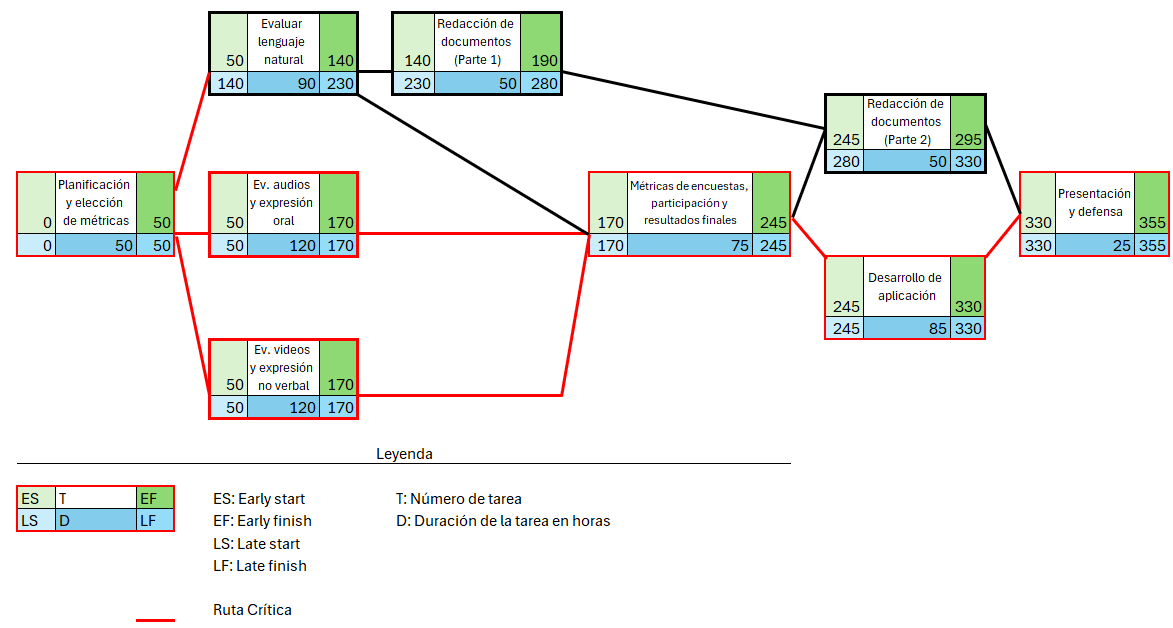
\includegraphics[width=1\textwidth]{./Figuras/Diagrama_AoN.png}
\caption{Diagrama de \textit{Activity on Node}.}
\label{fig:AoN}
\end{figure}

Como se puede observar, la ruta crítica empieza por la planificación luego hay un empate entre evaluar los audios y expresión oral vs. evaluar los videos y expresión no verbal. Cualquiera de los 2 modelos podría retrasar el desarrollo del proyecto. Posteriormente, sigue el desarrollo de las métricas adicionales y resultados finales, el desarrollo de la aplicación, y la presentación y defensa.

Cabe resaltar que este diagrama muestra que el proyecto se podría completar en menos tiempo (355 horas) pero en un escenario donde se tendrían que trabajar tres modelos en paralelo, lo que exigiría más de una persona trabajando en el proyecto. Debido a que esto no se cumple ya que el proyecto está a cargo de una sola persona, en la siguiente sección, se muestra el diagrama de Gantt considerando un avance en su mayoría serial y no paralelo.

\section{11. Diagrama de Gantt}
\label{sec:gantt}

A continuación, en la figura \ref{fig:diagGantt}, se muestra el diagrama de Gantt del proyecto.

\begin{landscape}
\begin{figure}[htpb]
\centering 
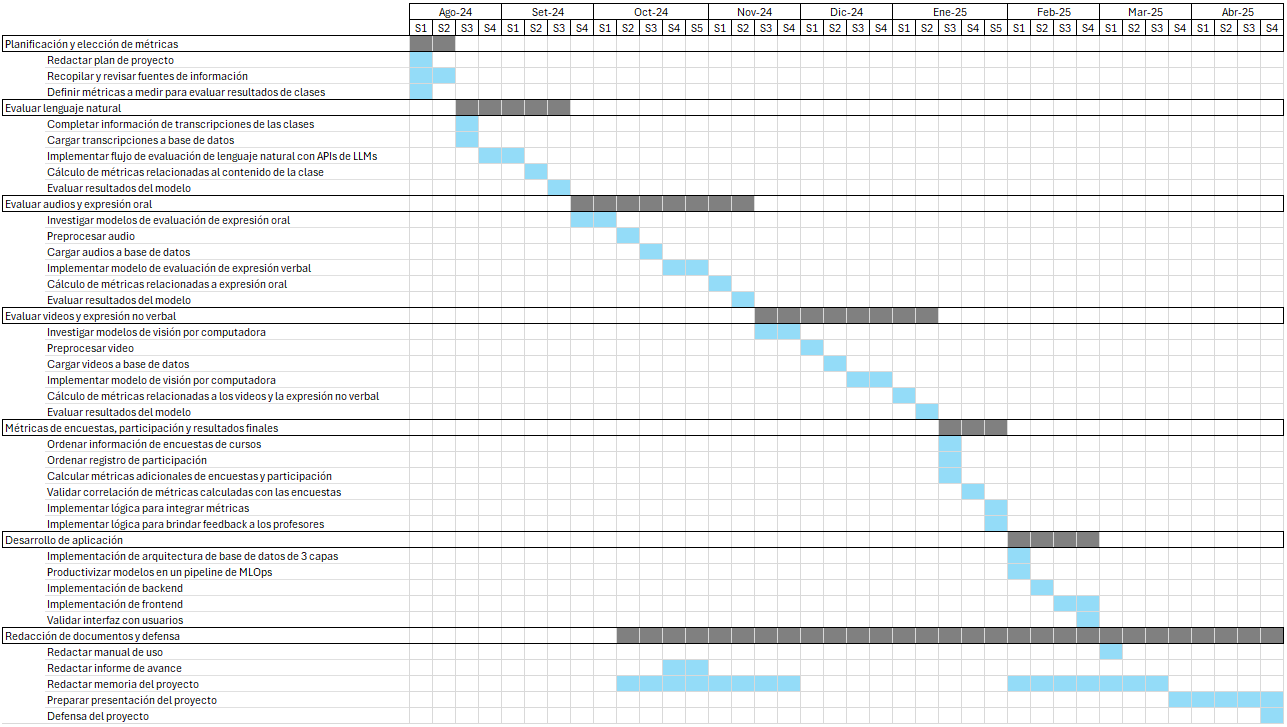
\includegraphics[height=.9\textheight]{./Figuras/diagrama_gantt.png}
\caption{Diagrama de Gantt} %Modificar este título acorde.
\label{fig:diagGantt}
\end{figure}

\end{landscape}


\section{12. Presupuesto detallado del proyecto}
\label{sec:presupuesto}

En esta sección, se enlistan los costos asociados al desarrollo del proyecto, separados por directos e indirectos:

\begin{table}[htpb]
\centering
\begin{tabularx}{\linewidth}{@{}|X|c|r|r|@{}}
\hline
\rowcolor[HTML]{C0C0C0} 
\multicolumn{4}{|c|}{\cellcolor[HTML]{C0C0C0}COSTOS DIRECTOS} \\ \hline
\rowcolor[HTML]{C0C0C0} 
Descripción &
  \multicolumn{1}{c|}{\cellcolor[HTML]{C0C0C0}Cantidad} &
  \multicolumn{1}{c|}{\cellcolor[HTML]{C0C0C0}Valor unitario} &
  \multicolumn{1}{c|}{\cellcolor[HTML]{C0C0C0}Valor total} \\ \hline
Mes de ingeniería trabajado &
  \multicolumn{1}{c|}{9 meses} &
  \multicolumn{1}{c|}{1500 USD} &
  \multicolumn{1}{c|}{13500 USD} \\ \hline
Créditos por uso de APIs de IAs preentrenadas &
  \multicolumn{1}{c|}{300 MM tokens} &
  \multicolumn{1}{c|}{0.15 USD x MM} &
  \multicolumn{1}{c|}{45 USD} \\ \hline
Servicios en la nube para pruebas &
  \multicolumn{1}{c|}{9 meses} &
  \multicolumn{1}{c|}{4.86 USD} &
  \multicolumn{1}{c|}{43.74 USD} \\ \hline
\multicolumn{3}{|c|}{SUBTOTAL} &
  \multicolumn{1}{c|}{13588.74 USD} \\ \hline
\rowcolor[HTML]{C0C0C0} 
\multicolumn{4}{|c|}{\cellcolor[HTML]{C0C0C0}COSTOS INDIRECTOS} \\ \hline
\rowcolor[HTML]{C0C0C0} 
Descripción &
  \multicolumn{1}{c|}{\cellcolor[HTML]{C0C0C0}Cantidad} &
  \multicolumn{1}{c|}{\cellcolor[HTML]{C0C0C0}Valor unitario} &
  \multicolumn{1}{c|}{\cellcolor[HTML]{C0C0C0}Valor total} \\ \hline
\multicolumn{1}{|l|}{Devaluación equipos de computación} &
   9 meses&
   30 USD &
   270 USD\\ \hline
\multicolumn{3}{|c|}{SUBTOTAL} &
  \multicolumn{1}{c|}{270 USD} \\ \hline
\rowcolor[HTML]{C0C0C0}
\multicolumn{3}{|c|}{TOTAL} &
   13858.74 USD\\ \hline
\end{tabularx}%
\end{table}


\section{13. Gestión de riesgos}
\label{sec:riesgos}

a) A continuación, se presentan los riesgos asociados al proyecto y su puntuación en relación a qué tan severo sería su impacto en el trabajo y cuán probable es que ocurra.
 
Riesgo 1: dificultad para procesar las transcripciones faltantes de las clases.
\begin{itemize}
	\item Severidad (S): 8, ya que esta información es el insumo principal de los modelos de lenguaje natural.
	\item Probabilidad de ocurrencia (O): 4, dado que existen diversas herramientas que se pueden probar para realizar las transcripciones.
\end{itemize}   

Riesgo 2: que el procesamiento de audio y video tome más tiempo del estimado.
\begin{itemize}
	\item Severidad (S): 8, ya que se puede priorizar uno u otro dato (o audio o video), pero se necesita al menos una de estas fuentes para tener un modelo robusto.
	\item Ocurrencia (O): 5, dado que son tipos de archivos más complicados para procesar que el texto.
\end{itemize}

Riesgo 3: que la cantidad necesaria de GPUs para el entrenamiento de los modelos sea mayor a la que se tiene actualmente.
\begin{itemize}
	\item Severidad (S): 8, ya que el poder de procesamiento es importante para culminar el proyecto.
	\item Ocurrencia (O): 3, dado que existen diferentes alternativas de renta de GPUs en la nube.
\end{itemize}

Riesgo 4: que no existan modelos preentrenados capaces de evaluar audio y video de la forma que se requiere.
\begin{itemize}
	\item Severidad (S): 6, porque va a ser importante tener modelos preentrenados para completar el trabajo a tiempo.
	\item Ocurrencia (O): 4, ya que continuamente salen más y mejores modelos al mercado para todo tipo de aplicaciones.
\end{itemize}

Riesgo 5: que las computadoras que se tienen disponibles fallen o sufran algún daño.
\begin{itemize}
	\item Severidad (S): 8, ya que son fundamentales para el desarrollo del proyecto.
	\item Ocurrencia (O): 2, dado que se cuenta con 2 computadoras y la información será guardada en la nube como respaldo.
\end{itemize}


b) Tabla de gestión de riesgos:      (El RPN se calcula como RPN=SxO)

\begin{table}[htpb]
\centering
\begin{tabularx}{\linewidth}{@{}|X|c|c|c|c|c|c|@{}}
\hline
\rowcolor[HTML]{C0C0C0} 
Riesgo & S & O & RPN & S* & O* & RPN* \\ \hline
      1: dificultad para procesar las transcripciones faltantes de las clases. &  8 &  4 &   32 &  8 &  2 & 16   \\ \hline
      2: que el procesamiento de audio y video tome más tiempo del estimado. &  8 &  5 &   40 &  8 &  3 & 24   \\ \hline
      3: que la cantidad necesaria de GPUs para el entrenamiento de los modelos sea mayor. &  8 &  3 &   24 &   &   &     \\ \hline
      4: que no existan modelos preentrenados capaces de evaluar audio y video de la forma que se requiere. &  6 &  4 &   24 &    &    &      \\ \hline
      5: que las computadoras que se tienen disponibles se malogren. &  8 &  2 &   16 &    &    &      \\ \hline
\end{tabularx}%
\end{table}

Criterio adoptado: 
se tomarán medidas de mitigación en los riesgos cuyos números de RPN sean mayores o iguales a 30.

c) Plan de mitigación de los riesgos que originalmente excedían el RPN máximo establecido:
 
Riesgo 1: se probarán diversas herramientas de transcripción para encontrar la mejor alternativa en tiempo y precio.
\begin{itemize}
  \item Severidad (S): 8, se mantiene.
  \item Probabilidad de ocurrencia (O): 2, la probabilidad de ocurrencia disminuye ya que se tendrá conocimiento de diferentes alternativas.
\end{itemize}

Riesgo 2: se buscará asesoramiento de expertos en procesamiento de audio y video.
\begin{itemize}
  \item Severidad (S): 8, se mantiene.
  \item Probabilidad de ocurrencia (O): 3, con la ayuda del experto se podrá encontrar el modelo más apropiado y óptimo en cuestión de tiempos de entrenamiento.
\end{itemize}
 

\section{14. Gestión de la calidad}
\label{sec:calidad}

En esta sección se presentan las acciones de verificación y validación de calidad de los requerimientos del proyecto.

\begin{enumerate}
	\item Requerimientos funcionales:
		\begin{enumerate}
			\item El sistema debe tener una base de datos que permita almacenar datos no estructurados y estructurados.
                    \begin{itemize}
                    	\item Verificar que los programas de bases de datos seleccionados permitan ambos tipos de datos.
                    	\item Validar con una prueba la carga de datos estructurados y no estructurados.
                    \end{itemize}
                \item La base de datos debe estar organizada de tal forma que se pueda diferenciar la data en bruto de la procesada. Para esto, se debe usar una arquitectura de base de datos de tres capas.
                    \begin{itemize}
                    	\item Verificar que la arquitectura cumpla con las tres capas requeridas.
                    	\item Validar que el flujo de información se procese y almacene correctamente en las diferentes capas.
                    \end{itemize}
			\item Se deben utilizar por lo menos tres fuentes de información.
                    \begin{itemize}
                    	\item Verificar la cantidad de fuentes de información utilizadas por los modelos.
                    	\item Validar que el modelo toma en cuenta patrones de diferentes fuentes de información para dar recomendaciones.
                    \end{itemize}
			\item Los resultados finales deben ser presentados de forma que sean fáciles de interpretar por los usuarios.
                    \begin{itemize}
                    	\item Verificar que los resultados se presenten de forma gráfica y resumida.
                    	\item Validar con un usuario que los resultados sean entendibles.
                    \end{itemize}
                \item El código en Python debe estar claro y ordenado de acuerdo a la buenas prácticas de programación.
                    \begin{itemize}
                    	\item Releer el código para verificar que se cumplan las buenas prácticas.
                    	\item Validar con el director si es que el código es entendible y ordenado.
                    \end{itemize}
                \item Los modelos deben ser desplegados en un pipeline de MLOps.
                    \begin{itemize}
                    	\item Verificar el diseño e implementación de un pipeline de MLOps.
                    	\item Validar que el modelo se pueda ejecutar en producción de forma automática y sin errores.
                    \end{itemize}
                \item Se debe construir un API que permita hacer consultas a los modelos desde la capa de aplicación del usuario.
                   \begin{itemize}
                    	\item Verificar el uso de un API dentro del pipeline de MLOps.
                    	\item Validar que se puedan hacer inferencias con el modelo correctamente mediante el API.
                    \end{itemize}
            \end{enumerate}
	\item Requerimientos de documentación:
		\begin{enumerate}
			\item Se debe crear una guía de usuario que explique cómo utilizar la herramienta.
                 \begin{itemize}
                    	\item Verificar la creación de una guía de usuario.
                    	\item Validar con el cliente que la guía le sirva para aprender a usar la herramienta sin inconvenientes.
                    \end{itemize}
		\end{enumerate}
	\item Requerimientos de la interfaz
 		\begin{enumerate}
			\item Se debe crear una aplicación web con una interfaz fácil de usar que muestre los resultados finales y recomendaciones. Se debe utilizar los conocimientos de Angular y/o Ionic.
                 \begin{itemize}
                    	\item Verificar la creación de una web con interfaz sencilla.
                    	\item Validar con el cliente que la web le funcione correctamente y sea fácil de usar.
                    \end{itemize}
		\end{enumerate}

\end{enumerate}

\section{15. Procesos de cierre}    
\label{sec:cierre}


Se establecen las siguientes pautas de trabajo para realizar una reunión final de evaluación del proyecto, tal que contemple las siguientes actividades:

\begin{itemize}
	\item Evaluar si los requerimientos estipulados se cumplieron:\\
	 - A cargo del cliente y del director
	\item Identificar las técnicas y procedimientos útiles e inútiles que se emplearon, los problemas que surgieron y cómo se solucionaron:\\
	 - A cargo de la responsable del proyecto.
	\item Organizar el acto de agradecimiento a todos los interesados, y en especial al equipo de trabajo y colaboradores:\\
	  - A cargo de la responsable del proyecto.
\end{itemize}


\end{document}